\begin{frame}{Canonical search problem $\Search_{\varphi}$ (Impagliazzo et al. 1994)}

	
    $\varphi(x, y)$ is an unsatisfiable CNF formula:
    \begin{itemize}
        \item Alice receives a substitution to the variables $x$, Bob receives a substitution to the
            variables $y$;
        \item goal is to find a clause $C \in \varphi$ that is unsatisfied by this substitution.
    \end{itemize}

    \pause

    \begin{theorem}[Beame, Pitassi, Segerlind 2007. Informal]
        If there is a {\color{blue} tree-like} proof in proof system $\Pi$ ($\Pi$ from some \textit{huge
          class}) of size $S$ then there is a communication protocol for $\Search_{\varphi}$ of depth
        $poly(\log(S))$.
    \end{theorem}
    
\end{frame}


\begin{frame}{Proofs and games}
	$D_1, D_2, \dots, D_{17}$ is a semantic proof of of $\varphi(x, y)$.

    \begin{center}
    	\tikzstyle{inner} = [thin, circle, minimum size = 0.6cm, draw, inner sep = 0.1pt, black, font = \scriptsize]
\tikzstyle{inner_g} = [thin, circle, minimum size = 0.6cm, draw, inner sep = 0.1pt, black, fill = green]
\tikzstyle{inner_r} = [thin, circle, minimum size = 0.6cm, draw, inner sep = 0.1pt, black, fill = red]
\tikzstyle{inner_b} = [
	thin, circle, minimum size = 0.6cm, draw, inner sep = 0.1pt, black, fill = blue!30!white, font =
    \scriptsize]
\tikzstyle{ed} = [thick, ->, draw, black]

    
\begin{tikzpicture}

    \only<-1>{
        \node[inner] (a) at (0, 0) {$D_{17}$};
	}
    \only<2->{
        \node[inner_b] (a) at (0, 0) {$D_{17}$};
    }

    \only<-2>{
        \node[inner] (b) at (-1.5, -1) {$D_{16}$};
	}
    \only<3->{
        \node[inner_b] (b) at (-1.5, -1) {$D_{16}$};
    }
  

    \node[inner] (c) at (1.5, -1) {$D_{15}$};

    \node[inner] (d) at (-3, -2) {$D_{14}$};

    \only<-3>{
        \node[inner] (e) at (0, -2) {$D_{13}$};
	}
    \only<4->{
        \node[inner_b] (e) at (0, -2) {$D_{13}$};
    }

    \node[inner] (f) at (3, -2) {$D_{12}$};

    \node[inner] (g) at (-4.5, -3) {$D_{11}$};

    \only<-4>{
        \node[inner] (h) at (-1.5, -3) {$D_{10}$};
	}
    \only<5->{
        \node[inner_b] (h) at (-1.5, -3) {$D_{10}$};
    }

    \node[inner] (i) at (1.0, -3) {$D_9$};

    \only<-6>{
        \node[inner] (j) at (2.0, -3) {$D_8$};
	}
    \only<7->{
        \node[inner_b] (j) at (2.0, -3) {$D_8$};
    }

    \node[inner] (k) at (4.0, -3) {$D_7$};

    \only<-5>{
        \node[inner] (l) at (-2.5, -4) {$D_6$};
	}
    \only<6->{
        \node[inner_b] (l) at (-2.5, -4) {$D_6$};
    }

    \node[inner] (m) at (-0.5, -4) {$D_5$};

    \only<-7>{
        \node[inner] (n) at (1.2, -4) {$D_4$};
	}
    \only<8->{
        \node[inner_b] (n) at (1.2, -4) {$D_4$};
    }

    \node[inner] (o) at (2.8, -4) {$D_3$};

    \node[inner] (p) at (0.4, -5) {$D_2$};
    
    \only<-8>{
        \node[inner] (q) at (2, -5) {$D_1$};
	}
    \only<9->{
        \node[inner_b] (q) at (2, -5) {$D_1$};
    }


    
    \path (a) edge[ed] (b);
    \path (a) edge[ed] (c);
    \path (b) edge[ed] (d);
    \path (b) edge[ed] (e);
    \path (c) edge[ed] (e);
    \path (c) edge[ed] (f);
    \path (d) edge[ed] (g);
    \path (d) edge[ed] (h);
    \path (e) edge[ed] (h);
    \path (e) edge[ed] (i);
    \path (f) edge[ed] (j);
    \path (f) edge[ed] (k);
    \path (h) edge[ed] (l);
    \path (h) edge[ed] (m);
    \path (j) edge[ed] (n);
    \path (j) edge[ed] (o);
    \path (n) edge[ed] (p);
    \path (n) edge[ed] (q);
\end{tikzpicture}
    
    \end{center}

    \pause
    Size of game is the size of graph. Coomunication complexity of game is the comunication complexity of
    evaluation of constaint.

\end{frame}


\begin{frame}{Games and circuits}

    A communication problem on sets $U, V \subseteq \{0, 1\}^{n}$ and relation $\Bit$:
    \begin{itemize}
        \item Alice receives $u \in U$, Bob receives $v \in V$;
        \item goal is to find $i$ such that $u_i \neq v_i$.
    \end{itemize}
    \pause
    Monotone case ($\MBit$ relation):
    \begin{itemize}
        \item goal is to find $i$ such that $u_i = 1 \land v_i = 0$.
    \end{itemize}

    \pause

    \vspace{0.2cm}
    $U = f^{-1}(1), V = f^{-1}(0)$

    \begin{itemize}
        \item {[Karchmer, Wigderson 1990]} Communication protocol of size $S$ for the relation $\Bit$
            \alert{$(\MBit)$} $\Leftrightarrow$ \alert{(monotone)} boolean formula for $f$ of size $S$.
        \pause
        \item {[Razborov 94]} Communication game of size $S$ and $CC = k$ for the relation $\Bit$
            \alert{$(\MBit)$} $\Leftrightarrow$ \alert{(monotone)} boolean circuit for $f$ of size $2^k
            S$.
    \end{itemize}
\end{frame}

\begin{frame}{Results}
    \begin{itemize}
        \item {[Karchmer, Wigderson 1990]} Communication protocol of size $S$ for the relation $\Bit$
            \alert{$(\MBit)$} $\Leftrightarrow$ \alert{(monotone)} boolean formula for $f$ of size $S$.
        \item {[Razborov 94]} Communication game of size $S$ and $CC = k$ for the relation $\Bit$
            \alert{$(\MBit)$} $\Leftrightarrow$ \alert{(monotone)} boolean circuit for $f$ of size
            $2^{3k} S$.
        \pause
        \item {[Pudl{\'{a}}k 10, S 17]} Communication game of size $S$ and $CC = k$ for some relation $N$
            $\Leftrightarrow$ communication game of size $2^{3k} S$ and $CC = \frac{3}{2}$ (two
            independent rounds) for some relation $N$.
    \end{itemize}
    
    \vspace{0.3cm}
    \pause
    \begin{itemize}                
        \item {[S 17]} There are two $\NP$ sets such that any communication game of size $S$ and $RCC = 1$
            for the relation $\MBit$ has size at least $2^{n^{\frac{1}{8}}}$.
        \pause    
        \item {[Pudl{\'{a}}k, Hrube{\v{s}} 17]} Communication game of size $S$ and $RCC = 1$ for the
            relation $\MBit$ $\Leftrightarrow$ monotone {\color{blue} real}
            circuit for $f$ of size $O(S)$.
    \end{itemize}
\end{frame}
    


\begin{frame}{$\MBit \le \Search_{\varphi}$}


\end{frame}


\begin{frame}{$\MBit \le \Search_{\varphi}$}

	Случайные формулы.  Pit and Pud.
\end{frame}